\documentclass[conference]{IEEEtran}
\usepackage{graphicx,booktabs,amsmath,cite,url}
\begin{document}
\title{Automatic Short-Answer Scoring for a Secure Digital Evaluation System: A Comparative Study of Classical Machine Learning and Large Language Models on ASAP-SAS}
\author{\IEEEauthorblockN{Shaik Naveed Ahamed}
\IEEEauthorblockA{School of Computer Science and Engineering\\REVA University, Bengaluru, India}}
\maketitle

\begin{abstract}
Manual evaluation of examination answer scripts is slow, costly and prone to inconsistency between markers. We present a Digital Evaluation System (DES) that digitises the full evaluation pipeline -- secure script access, anonymised evaluator assignment, online marking, moderation, automated tabulation and result publication -- and augments it with a machine-learning assistant that proposes a mark for each answer. To choose the scoring model, we benchmark five supervised learners (Ridge regression, logistic regression, linear SVM, random forest, XGBoost) on TF-IDF and handcrafted features against a zero-shot large language model (LLM) scoring from the rubric alone, using the public ASAP Short Answer Scoring dataset (13,634 human-scored answers, 10 prompts). Logistic Regression achieves the highest quadratic weighted kappa (QWK = 0.662) on a stratified hold-out set, against a human inter-rater agreement of 0.906; 5-fold cross-validation confirms its stability (QWK = 0.661 $\pm$ 0.005). On a common 200-answer sample, the zero-shot LLM reaches QWK = 0.541 without any training data, versus 0.606 for the best trained model. Because neither approach reaches human agreement, the DES uses model output strictly as an advisory suggestion that an evaluator must confirm, keeping humans accountable for every mark.
\end{abstract}
\begin{IEEEkeywords}automatic short answer grading, digital evaluation, quadratic weighted kappa, machine learning, large language models, educational assessment\end{IEEEkeywords}

\section{Introduction}
Universities evaluate millions of handwritten answer scripts every semester. The traditional process -- physically moving scripts to evaluators, totalling marks by hand, and transcribing them into result sheets -- is time-consuming, error-prone and difficult to audit. On-screen (digital) evaluation addresses logistics and transparency, but marking consistency still depends entirely on individual evaluators.

Automatic short-answer grading (ASAG) has been studied for over two decades \cite{burrows2015}. The 2012 Hewlett Foundation ASAP competition released a public benchmark of short constructed responses with double human scoring \cite{shermis2014}, enabling reproducible comparison. Recently, LLMs have made rubric-based scoring possible without task-specific training data.

This paper makes three contributions: (1) the design and implementation of a role-based Digital Evaluation System with an integrated, human-in-the-loop scoring assistant; (2) a reproducible comparison of five classical learners on ASAP-SAS, with hold-out, cross-validation and learning-curve analyses; and (3) a same-sample comparison between trained models and a zero-shot LLM, which motivates the advisory-only design adopted in the system.

\section{Related Work}
Burrows et al.\ \cite{burrows2015} survey ASAG and group methods into concept mapping, information extraction, corpus-based, machine-learning and evaluation eras. Mohler and Mihalcea \cite{mohler2009} showed that corpus-based semantic similarity to a reference answer correlates with human grades. On ASAP-SAS, feature-rich supervised models remain strong baselines; Kumar et al.\ \cite{kumar2019} combine lexical, semantic and prompt-specific features (AutoSAS), while Riordan et al.\ \cite{riordan2017} study neural architectures for short-answer scoring. Transformer encoders such as BERT \cite{devlin2019} further improve accuracy but require GPU training per prompt. QWK \cite{cohen1968} is the standard agreement metric for this task. Our work differs by evaluating models in the context of an operational evaluation workflow and by comparing them with LLM rubric scoring on identical answers.

\section{System Architecture}
The DES is a web application with four roles. The \emph{Controller} (administrator) creates examinations and questions with maximum marks and model answers, uploads scanned scripts to private storage, and assigns them to evaluators and moderators. \emph{Evaluators} see only anonymised script codes, enter marks and remarks per question, save drafts and submit. \emph{Moderators} review submitted scripts and may change marks only with a recorded reason, producing an audit trail. After moderation, the Controller publishes results, and \emph{students} see their marks and grades.

Security is enforced in the database: row-level security policies restrict each role to its own records; student identity is stored separately from scripts so that markers cannot de-anonymise them; and every workflow write (assignment, marking, moderation, publication) passes through server-side functions that validate role, ownership and mark limits. An analytics module additionally runs Isolation Forest \cite{liu2008} over marking data in a separate Python service to flag unusual marking for moderator review.

The scoring assistant sends the question, model answer, maximum marks and the student's answer to the scoring model and displays a suggested mark with a short justification beside the mark field. The suggestion is never written automatically; the evaluator must enter or accept the mark, and the value is clamped to the question's limit.

\section{Dataset and Methodology}
\subsection{Dataset}
We use ASAP-SAS \cite{shermis2014}, comprising answers from US Grade 10 students to 10 prompts across science, biology and English language arts. We combine the officially released labelled training and validation portions (13,634 answers; Table~\ref{tab:data}), and use rater 1 (Score1) as the gold label. Rater 2 provides the human agreement ceiling.

\begin{table}[t]\centering\caption{ASAP-SAS prompts used}\label{tab:data}
\begin{tabular}{ccccc}\toprule
Set & Answers & Range & Mean score & Mean words \\\midrule
1 & 1328 & 0--3 & 1.49 & 47.6 \\
2 & 1031 & 0--3 & 1.72 & 59.4 \\
3 & 1451 & 0--2 & 0.94 & 47.6 \\
4 & 1316 & 0--2 & 0.69 & 40.1 \\
5 & 1431 & 0--3 & 0.28 & 24.6 \\
6 & 1423 & 0--3 & 0.24 & 23.5 \\
7 & 1441 & 0--2 & 0.71 & 41.5 \\
8 & 1461 & 0--2 & 1.13 & 53.0 \\
9 & 1434 & 0--2 & 1.09 & 49.5 \\
10 & 1318 & 0--2 & 1.17 & 41.4 \\
\bottomrule\end{tabular}\end{table}

\subsection{Features}
For each prompt we fit (i) word 1--2-gram TF-IDF, (ii) character 2--5-gram TF-IDF (10,000 features), and (iii) seven handcrafted features: character and word length, type--token ratio, mean word length, sentence count, and absolute and relative overlap with content words of the prompt. Linear models use the sparse concatenation; tree models use 100 truncated-SVD components plus the handcrafted features. All transformations are fitted on training data only.

\subsection{Models}
One model per prompt is trained, as in the ASAP competition: a majority-class baseline; Ridge regression with outputs rounded and clipped to the valid score range; multinomial logistic regression ($C=4$); linear SVM ($C=0.5$); random forest (300 trees, class-balanced); and XGBoost \cite{chen2016} (250 trees, depth 5, learning rate 0.08). Implementations use scikit-learn \cite{pedregosa2011}.

For the LLM condition, a stratified sample of 20 hold-out answers per prompt (200 total) is scored zero-shot by a general-purpose LLM (\texttt{gpt-6-astra}) given only the prompt text with its rubric, the maximum score and the answer, with structured integer output.

\subsection{Evaluation protocol and metrics}
Each prompt is split 80/20 with stratification by score (seed 42). We report QWK (averaged across prompts with Fisher's $z$-transformation, following ASAP), accuracy, macro-F1 and RMSE. Robustness is assessed with stratified 5-fold cross-validation for the two strongest models, and data efficiency with a learning curve using 10--100\% of the training split.

\section{Results}
\subsection{Model comparison}
Table~\ref{tab:overall} and Fig.~\ref{fig:cmp} summarise hold-out performance. All learned models substantially exceed the majority baseline (QWK 0). Logistic Regression performs best (QWK 0.662, accuracy 0.702), closely followed by Ridge regression, while Random Forest on dense SVD features is weakest (QWK 0.554), indicating that sparse lexical features carry most of the signal for these prompts. A gap of 0.243 QWK remains to human agreement (0.906).

\begin{table}[t]\centering\caption{Overall hold-out results (2,733 answers)}\label{tab:overall}
\begin{tabular}{lcccc}\toprule
Model & QWK & Acc. & Macro-F1 & RMSE \\\midrule
Majority & 0.000 & 0.525 & 0.201 & 0.865 \\
Ridge & 0.654 & 0.670 & 0.585 & 0.590 \\
\textbf{Logistic Regression} & 0.662 & 0.702 & 0.611 & 0.618 \\
Linear SVM & 0.643 & 0.698 & 0.597 & 0.632 \\
Random Forest & 0.554 & 0.676 & 0.536 & 0.681 \\
XGBoost & 0.637 & 0.693 & 0.602 & 0.640 \\
Human rater 2 & 0.906 & 0.874 & 0.857 & 0.348 \\
\bottomrule\end{tabular}\end{table}

\begin{figure}[t]\centering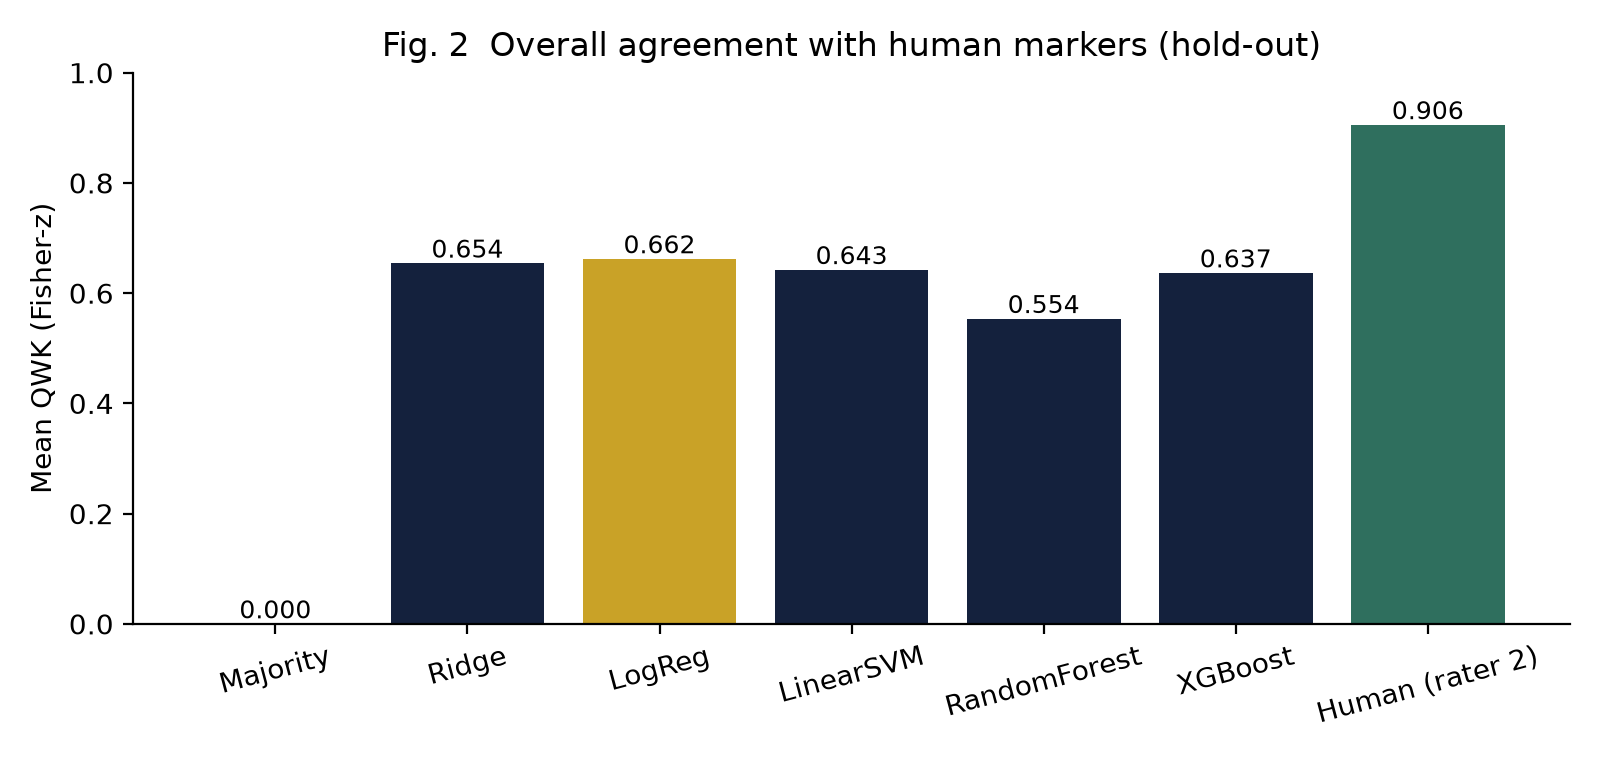
\includegraphics[width=\columnwidth]{fig2_model_comparison.png}
\caption{Mean QWK by model on the hold-out split.}\label{fig:cmp}\end{figure}

\subsection{Per-prompt analysis}
Performance varies considerably by prompt (Table~\ref{tab:perset}, Fig.~\ref{fig:perset}). For Logistic Regression, QWK ranges from 0.569 (set 2) to 0.750 (set 6). Prompts whose human agreement is itself low (sets 3 and 4, both 0.74) are also hard for the models, suggesting that rubric ambiguity limits achievable agreement.

\begin{table*}[t]\centering\caption{QWK per prompt on the hold-out split}\label{tab:perset}
\begin{tabular}{cc cccccc}\toprule
Set & Max & Ridge & Logistic Reg. & Linear SVM & Random Forest & XGBoost & Human \\\midrule
1 & 3 & 0.722 & 0.704 & 0.714 & 0.607 & 0.649 & 0.955 \\
2 & 3 & 0.592 & 0.569 & 0.569 & 0.481 & 0.539 & 0.895 \\
3 & 2 & 0.672 & 0.613 & 0.569 & 0.531 & 0.534 & 0.737 \\
4 & 2 & 0.599 & 0.623 & 0.626 & 0.592 & 0.603 & 0.735 \\
5 & 3 & 0.750 & 0.675 & 0.593 & 0.591 & 0.670 & 0.956 \\
6 & 3 & 0.760 & 0.750 & 0.714 & 0.399 & 0.780 & 0.961 \\
7 & 2 & 0.545 & 0.689 & 0.683 & 0.480 & 0.541 & 0.974 \\
8 & 2 & 0.600 & 0.587 & 0.600 & 0.482 & 0.585 & 0.853 \\
9 & 2 & 0.618 & 0.710 & 0.693 & 0.692 & 0.722 & 0.810 \\
10 & 2 & 0.625 & 0.665 & 0.631 & 0.625 & 0.671 & 0.885 \\
\bottomrule\end{tabular}\end{table*}

\begin{figure*}[t]\centering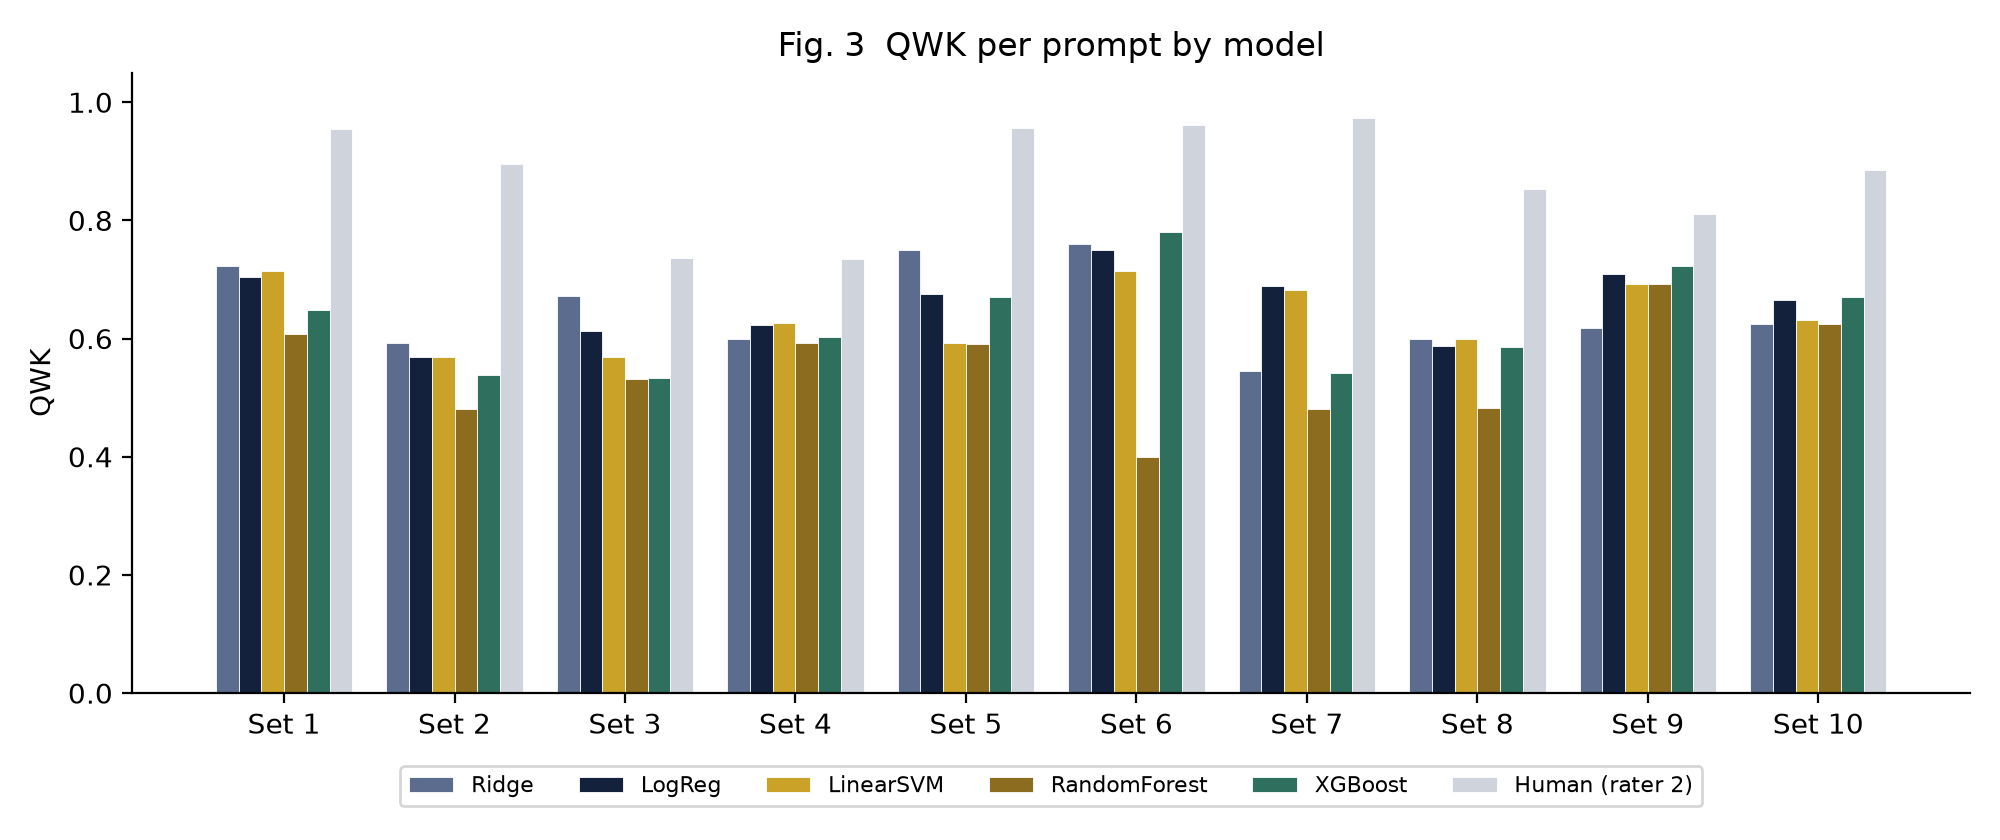
\includegraphics[width=0.85\textwidth]{fig3_qwk_per_prompt.png}
\caption{QWK per prompt for each model and for the second human rater.}\label{fig:perset}\end{figure*}

\subsection{Robustness and data efficiency}
Five-fold cross-validation (Table~\ref{tab:cv}) gives results consistent with the hold-out split, with low variance across folds. The learning curve (Table~\ref{tab:lc}, Fig.~\ref{fig:lc}) shows QWK rising from 0.519 with about 109 marked answers per prompt to 0.662 with about 1090; using 40\% of the data (about 436 answers) already reaches 0.617. In practice, an institution must mark several hundred answers per question before a trained model becomes useful.

\begin{table}[t]\centering\caption{Stratified 5-fold cross-validation}\label{tab:cv}
\begin{tabular}{lcc}\toprule Model & Mean QWK & Std \\\midrule
Logistic Regression & 0.661 & 0.005 \\
Ridge & 0.658 & 0.007 \\
\bottomrule\end{tabular}\end{table}

\begin{table}[t]\centering\caption{Learning curve for Logistic Regression}\label{tab:lc}
\begin{tabular}{ccc}\toprule Training data & Answers / prompt & QWK \\\midrule
10\% & 109 & 0.519 \\
20\% & 218 & 0.558 \\
40\% & 436 & 0.617 \\
60\% & 654 & 0.643 \\
80\% & 872 & 0.662 \\
100\% & 1090 & 0.662 \\
\bottomrule\end{tabular}\end{table}

\begin{figure}[t]\centering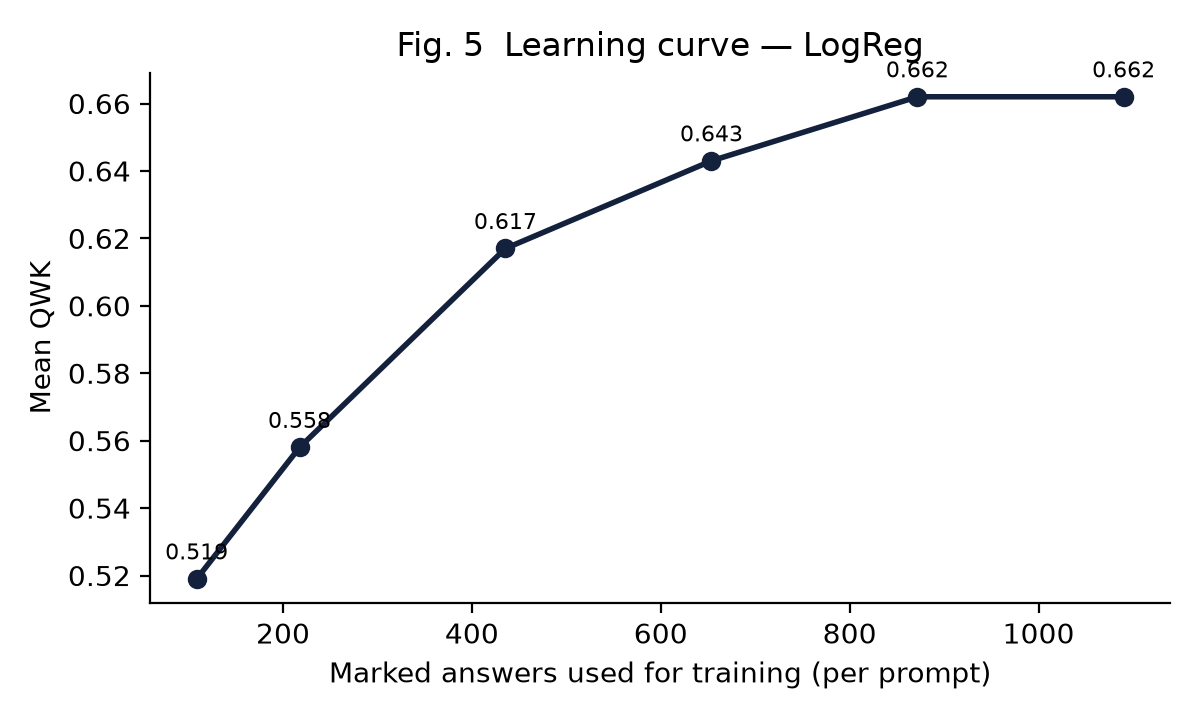
\includegraphics[width=\columnwidth]{fig5_learning_curve.png}
\caption{Learning curve: QWK vs.\ number of marked training answers.}\label{fig:lc}\end{figure}

\begin{figure}[t]\centering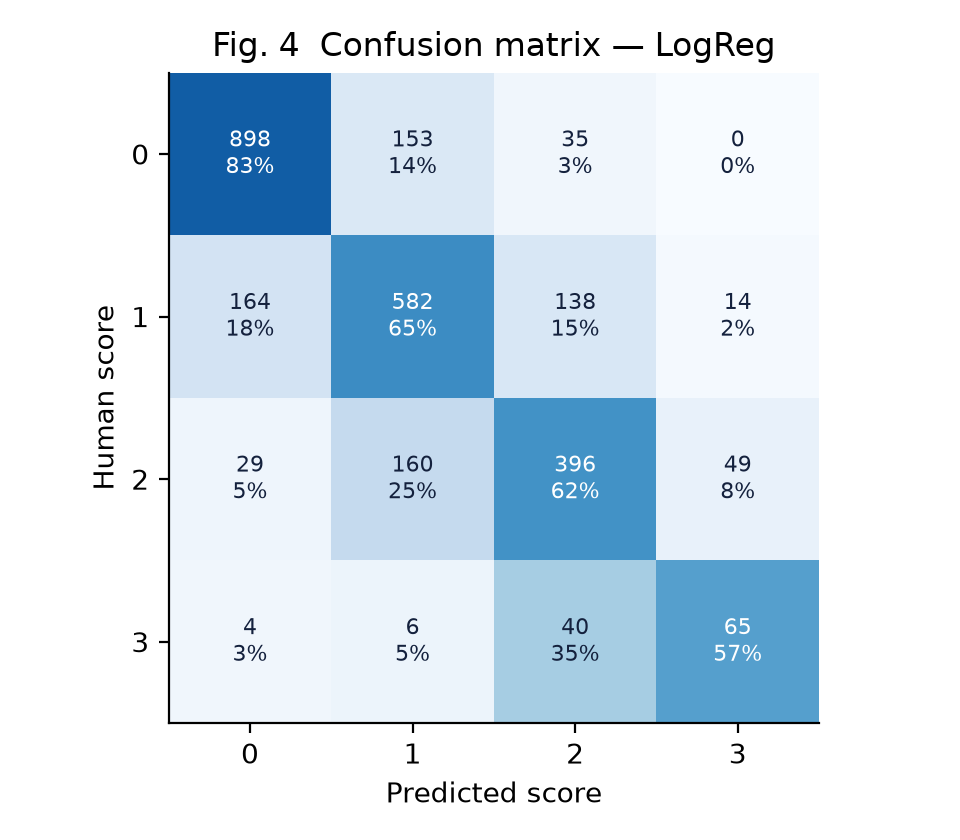
\includegraphics[width=0.8\columnwidth]{fig4_confusion_matrix.png}
\caption{Confusion matrix of Logistic Regression predictions (all prompts).}\label{fig:cm}\end{figure}

\subsection{Trained models vs.\ zero-shot LLM}
On the common 200-answer sample (Table~\ref{tab:llm}, Fig.~\ref{fig:llm}), the LLM obtains QWK 0.541 without seeing any labelled examples, compared with 0.606 for the best trained model (Logistic Regression) and 0.931 for the second human rater. The LLM's advantage is that it needs only the question and rubric, so it can assist from the first script of a new examination, whereas trained models require hundreds of marked answers per question. The trained models' advantage is higher agreement once such data exist, deterministic output, and negligible inference cost. The sample of 200 answers is small, so this comparison should be read as indicative.

\begin{table}[t]\centering\caption{Same-sample comparison (200 hold-out answers)}\label{tab:llm}
\begin{tabular}{lcc}\toprule Scorer & QWK & Acc. \\\midrule
Ridge & 0.552 & 0.625 \\
Logistic Regression & 0.606 & 0.690 \\
Linear SVM & 0.584 & 0.680 \\
Random Forest & 0.533 & 0.685 \\
XGBoost & 0.531 & 0.680 \\
LLM, zero-shot rubric & 0.541 & 0.550 \\
Human rater 2 & 0.931 & 0.870 \\
\bottomrule\end{tabular}\end{table}

\begin{figure}[t]\centering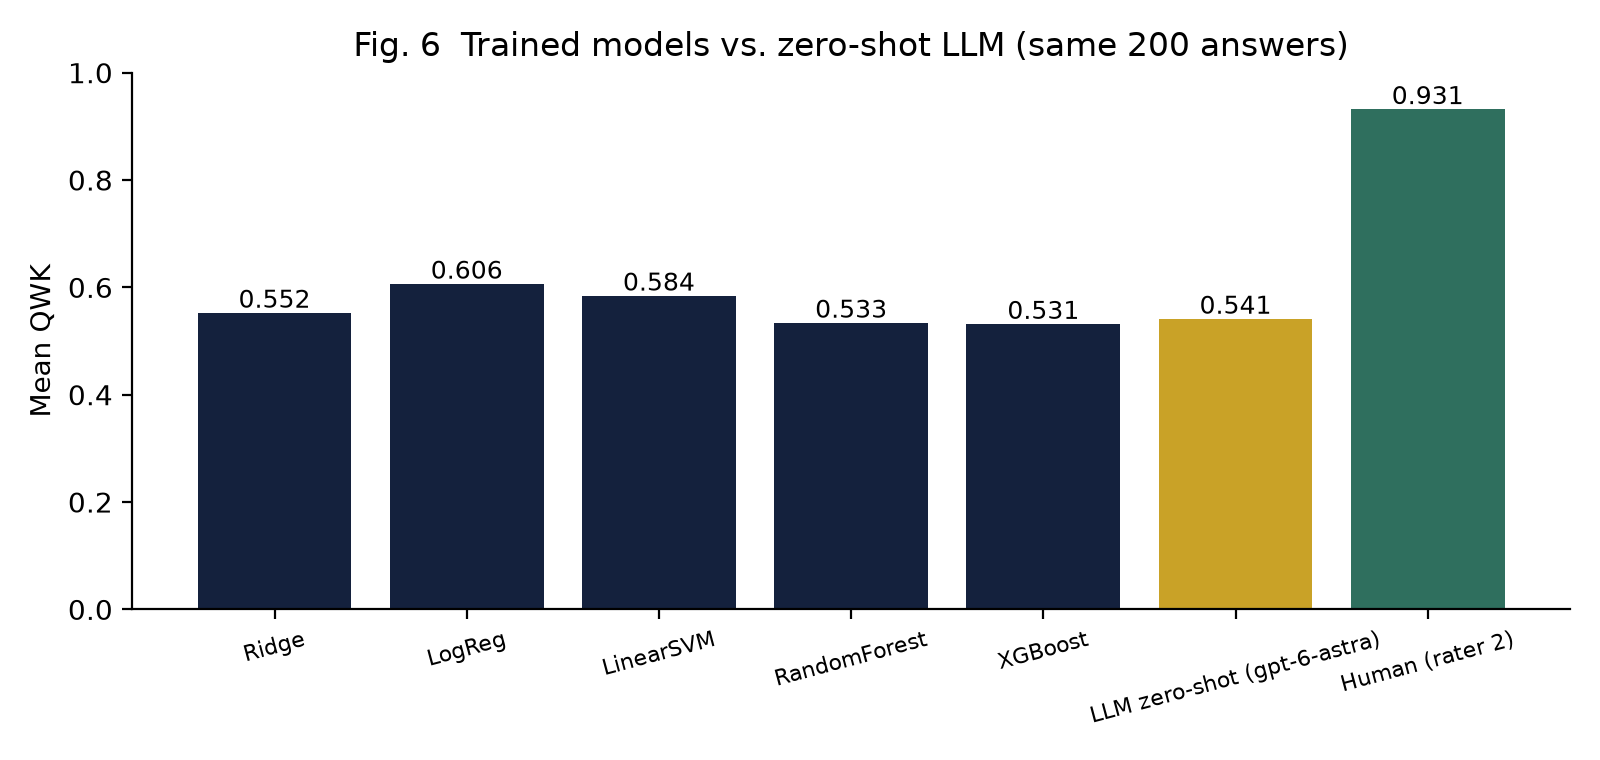
\includegraphics[width=\columnwidth]{fig6_llm_comparison.png}
\caption{Trained models vs.\ zero-shot LLM on the same 200 answers.}\label{fig:llm}\end{figure}

\section{Discussion}
No automatic scorer reached human-level agreement. For high-stakes examinations, we therefore integrate scoring as decision support: the evaluator sees a suggested mark and justification, but only a human-entered mark is stored, every moderation change requires a reason, and all actions are logged. This preserves accountability while still offering a consistency check that can surface overlooked content or unusually harsh or lenient marking. A practical deployment strategy is to start with LLM rubric scoring for new questions and switch to, or ensemble with, a trained model once enough moderated marks have accumulated in the DES database.

\section{Limitations and Future Work}
ASAP-SAS consists of typed English answers from US secondary students; our institution's scripts are handwritten and require OCR, whose errors are not modelled here. The LLM was evaluated on a 200-answer sample with a single prompt template. We did not fine-tune transformer encoders, which are known to outperform classical models on this benchmark. Future work will (i) collect and anonymise answers from REVA University examinations, (ii) evaluate OCR robustness, (iii) fine-tune transformer models and few-shot LLM prompts, and (iv) measure the effect of suggestions on evaluator time and consistency in a controlled study.

\section{Conclusion}
We presented a secure Digital Evaluation System and an empirical study of automatic short-answer scoring on ASAP-SAS. Logistic Regression on TF-IDF features was the strongest classical model (QWK 0.662), and a zero-shot LLM reached moderate agreement (0.541) without training data. Since both remain below human agreement (0.906), the system keeps humans in control and uses machine learning to support, not replace, examiners.

\section*{Reproducibility}
All code (experiment notebook, LLM evaluation script and system source) and the exact train/test split identifiers are available from the authors. Experiments use fixed random seeds.

\begin{thebibliography}{10}
\bibitem{burrows2015} S.~Burrows, I.~Gurevych, and B.~Stein, ``The eras and trends of automatic short answer grading,'' \emph{Int. J. Artif. Intell. Educ.}, vol.~25, no.~1, pp.~60--117, 2015.
\bibitem{shermis2014} M.~D.~Shermis, ``State-of-the-art automated essay scoring: Competition, results, and future directions from a United States demonstration,'' \emph{Assessing Writing}, vol.~20, pp.~53--76, 2014.
\bibitem{mohler2009} M.~Mohler and R.~Mihalcea, ``Text-to-text semantic similarity for automatic short answer grading,'' in \emph{Proc. EACL}, 2009, pp.~567--575.
\bibitem{kumar2019} Y.~Kumar, S.~Aggarwal, D.~Mahata, R.~R.~Shah, P.~Kumaraguru, and R.~Zimmermann, ``Get IT scored using AutoSAS -- An automated system for scoring short answers,'' in \emph{Proc. AAAI}, 2019, pp.~9662--9669.
\bibitem{riordan2017} B.~Riordan, A.~Horbach, A.~Cahill, T.~Zesch, and C.~M.~Lee, ``Investigating neural architectures for short answer scoring,'' in \emph{Proc. 12th Workshop on Innovative Use of NLP for Building Educational Applications}, 2017, pp.~159--168.
\bibitem{devlin2019} J.~Devlin, M.-W.~Chang, K.~Lee, and K.~Toutanova, ``BERT: Pre-training of deep bidirectional transformers for language understanding,'' in \emph{Proc. NAACL-HLT}, 2019, pp.~4171--4186.
\bibitem{cohen1968} J.~Cohen, ``Weighted kappa: Nominal scale agreement provision for scaled disagreement or partial credit,'' \emph{Psychological Bulletin}, vol.~70, no.~4, pp.~213--220, 1968.
\bibitem{liu2008} F.~T.~Liu, K.~M.~Ting, and Z.-H.~Zhou, ``Isolation forest,'' in \emph{Proc. IEEE ICDM}, 2008, pp.~413--422.
\bibitem{chen2016} T.~Chen and C.~Guestrin, ``XGBoost: A scalable tree boosting system,'' in \emph{Proc. ACM SIGKDD}, 2016, pp.~785--794.
\bibitem{pedregosa2011} F.~Pedregosa \emph{et al.}, ``Scikit-learn: Machine learning in Python,'' \emph{J. Mach. Learn. Res.}, vol.~12, pp.~2825--2830, 2011.
\end{thebibliography}
\end{document}
